\def\DoNotLoadEpstopdf{}
\documentclass[tikz,border=4pt]{standalone}
% Shared style for the technical appendix figures (2026-10-26).
% Builds on the proposal's figstyle.tex (same fonts, colors, and box styles) and adds
% one encoding for development status, used the same way in every appendix figure.
%   built and tested   solid border (the proposal's normal box styles)
%   built, no test     solid border, and the box text says "no test"
%   specified          dashed border            -> add the key  spec
%   planned            dotted grey border        -> use the style planned
%   no code (by hand)  dotted arrow              -> add the key  byhand
%   outside the artifact  solid grey border      -> use the style outside
% Shared style for proposal figures (2026-10-22 visuals pass).
% Sized to print at 6.5 in (16.5 cm) wide; body text 9 pt sans, nothing below 8 pt.
\usepackage[T1]{fontenc}
\usepackage[scaled=0.95]{helvet}
\renewcommand{\familydefault}{\sfdefault}
\usepackage{xcolor}
\usetikzlibrary{arrows.meta,positioning,calc,patterns.meta}
\definecolor{cink}{HTML}{16191F}
\definecolor{cmuted}{HTML}{4B5563}
\definecolor{cslate}{HTML}{2F4858}
\definecolor{cslatefill}{HTML}{E9EFF3}
\definecolor{cbrass}{HTML}{7A5C12}
\definecolor{cbrassfill}{HTML}{F5EFDE}
\definecolor{cred}{HTML}{8C2F39}
\definecolor{credfill}{HTML}{F8E9EA}
\definecolor{cgreen}{HTML}{235C53}
\definecolor{cgreenfill}{HTML}{E3F0EC}
\definecolor{caudit}{HTML}{5B3A8E}
\definecolor{cauditfill}{HTML}{EFE9F6}
\definecolor{cghost}{HTML}{6B7280}
\definecolor{cghostfill}{HTML}{F3F4F6}
\tikzset{
  >={Triangle[length=5pt,width=4.5pt]},
  box/.style={draw, rounded corners=1.5pt, line width=0.8pt, align=center, inner sep=4pt, font=\fontsize{9}{11}\selectfont},
  sub/.style={font=\fontsize{8}{9.6}\selectfont, text=cmuted},
  ai/.style={box, draw=cbrass, fill=cbrassfill, text=cbrass},
  ver/.style={box, draw=cred, fill=credfill, text=cred},
  pipe/.style={box, draw=cslate, fill=cslatefill, text=cslate},
  prod/.style={box, draw=cslate, fill=cslate, text=white},
  person/.style={box, draw=cink, fill=white, text=cink},
  ghost/.style={box, draw=cghost, fill=cghostfill, text=cghost, dash pattern=on 3pt off 2pt},
  flow/.style={->, line width=0.8pt},
}

\renewcommand{\ttdefault}{lmtt}% vector typewriter font (same design as the default, not a bitmap)
\tikzset{
  spec/.style={dash pattern=on 3pt off 2pt},
  planned/.style={box, draw=cghost, fill=cghostfill, text=cghost, dash pattern=on 0.9pt off 1.6pt},
  outside/.style={box, draw=cghost, fill=white, text=cghost},
  byhand/.style={dash pattern=on 0.9pt off 1.6pt},
  prog/.style={font=\fontsize{8}{9.6}\selectfont\ttfamily},
  legendbox/.style={draw, rounded corners=1pt, line width=0.8pt, minimum width=0.55cm, minimum height=0.32cm, inner sep=0pt},
  legendtext/.style={font=\fontsize{8}{9.6}\selectfont, text=cink, anchor=west, inner sep=1pt},
}
% \statuslegend{x}{y} draws the four-item status legend with its left edge at (x,y).
\newcommand{\statuslegend}[2]{%
  \begin{scope}[shift={(#1,#2)}]
    \node[legendbox, draw=cink, fill=white] (lg1) at (0.275,0) {};
    \node[legendtext] at (0.65,0) {Built and tested};
    \node[legendbox, draw=cink, fill=white, spec] (lg2) at (3.35,0) {};
    \node[legendtext] at (3.725,0) {Specified};
    \node[legendbox, draw=cghost, fill=cghostfill, dash pattern=on 0.9pt off 1.6pt] (lg3) at (5.75,0) {};
    \node[legendtext] at (6.125,0) {Planned};
    \node[legendbox, draw=cghost, fill=white] (lg4) at (7.85,0) {};
    \node[legendtext] at (8.225,0) {Outside the research artifact};
  \end{scope}}

% Figure A4 of the 10/26d appendix: how the audit layer would capture, tag, and store each AI session,
% and what would read its databases. Design only, no status.
\begin{document}
\hyphenpenalty=10000
\frenchspacing
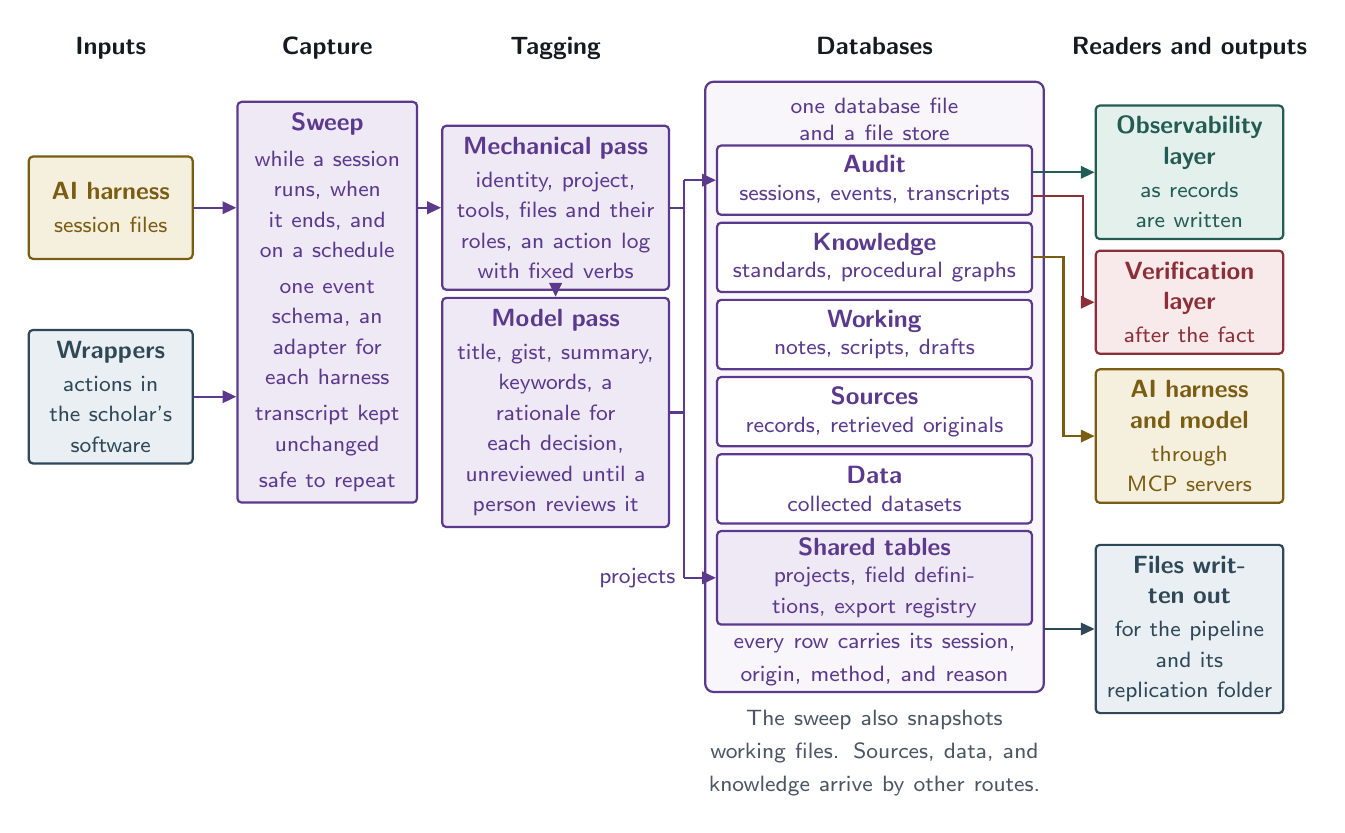
\begin{tikzpicture}
\tikzset{
  col/.style={font=\fontsize{9}{11}\selectfont\bfseries, text=cink, anchor=base},
  lab/.style={font=\fontsize{8}{9.4}\selectfont, inner sep=1.5pt},
  aud/.style={box, draw=caudit, fill=cauditfill, text=caudit},
  obs/.style={box, draw=cgreen, fill=cgreenfill, text=cgreen},
  store/.style={box, draw=caudit, fill=white, text=caudit, text width=3.8cm, minimum width=4.0cm, minimum height=0.88cm, inner sep=2.5pt},
}
\newcommand{\sm}[1]{{\fontsize{8}{9.4}\selectfont #1}}
\newcommand{\hd}[1]{{\fontsize{9}{11}\selectfont\bfseries #1}}
\def\dl{8.6}\def\dr{12.9}\def\dc{10.75}
% heads
\node[col] at (1.05,4.55) {Inputs};
\node[col] at (3.8,4.55) {Capture};
\node[col] at (6.7,4.55) {Tagging};
\node[col] at (\dc,4.55) {Databases};
\node[col] at (14.75,4.55) {Readers and outputs};
% inputs
\node[ai, text width=1.8cm, minimum width=2.0cm, minimum height=1.3cm] (hs) at (1.05,2.6) {\hd{AI harness}\\[1pt]\sm{session files}};
\node[pipe, text width=1.8cm, minimum width=2.0cm, minimum height=1.3cm] (wr) at (1.05,0.2) {\hd{Wrappers}\\[1pt]\sm{actions in the scholar's software}};
% capture
\node[aud, text width=2.0cm, minimum width=2.2cm, minimum height=3.9cm] (cap) at (3.8,1.4) {\hd{Sweep}\\[2pt]\sm{while a session runs, when it ends, and on a schedule}\\[2pt]\sm{one event schema, an adapter for each harness}\\[2pt]\sm{transcript kept unchanged}\\[2pt]\sm{safe to repeat}};
% tagging
\node[aud, text width=2.6cm, minimum width=2.8cm, minimum height=2.0cm] (mech) at (6.7,2.6) {\hd{Mechanical pass}\\[1pt]\sm{identity, project, tools, files and their roles, an action log with fixed verbs}};
\node[aud, text width=2.6cm, minimum width=2.8cm, minimum height=2.0cm] (llm) at (6.7,0.0) {\hd{Model pass}\\[1pt]\sm{title, gist, summary, keywords, a rationale for each decision, unreviewed until a person reviews it}};
% databases
\draw[caudit, line width=0.8pt, rounded corners=3pt, fill=cauditfill!40!white] (\dl,4.2) rectangle (\dr,-3.55);
\node[text=caudit, anchor=north, text width=4.1cm, align=center] at (\dc,4.12) {\sm{one database file}\\[-2pt]\sm{and a file store}};
\node[store] (sa) at (\dc,2.95) {\textbf{Audit}\\[-1pt]\sm{sessions, events, transcripts}};
\node[store] (sk) at (\dc,1.97) {\textbf{Knowledge}\\[-1pt]\sm{standards, procedural graphs}};
\node[store] (sw) at (\dc,0.99) {\textbf{Working}\\[-1pt]\sm{notes, scripts, drafts}};
\node[store] (ss) at (\dc,0.01) {\textbf{Sources}\\[-1pt]\sm{records, retrieved originals}};
\node[store] (sd) at (\dc,-0.97) {\textbf{Data}\\[-1pt]\sm{collected datasets}};
\node[store, fill=cauditfill, minimum height=1.0cm] (sh) at (\dc,-2.1) {\textbf{Shared tables}\\[-1pt]\sm{projects, field definitions, export registry}};
\node[text=caudit, text width=4.0cm, align=center, anchor=north] (foot) at (\dc,-2.68) {\sm{every row carries its session, origin, method, and reason}};
\node[text=cmuted, text width=4.3cm, align=center, anchor=north] at (\dc,-3.65) {\sm{The sweep also snapshots working files. Sources, data, and knowledge arrive by other routes.}};
% readers and outputs
\node[obs, text width=2.1cm, minimum width=2.3cm, minimum height=1.25cm] (ob) at (14.75,3.05) {\hd{Observability layer}\\[1pt]\sm{as records are written}};
\node[ver, text width=2.1cm, minimum width=2.3cm, minimum height=1.25cm] (ve) at (14.75,1.4) {\hd{Verification layer}\\[1pt]\sm{after the fact}};
\node[ai, text width=2.1cm, minimum width=2.3cm, minimum height=1.25cm] (mc) at (14.75,-0.3) {\hd{AI harness and model}\\[1pt]\sm{through MCP servers}};
\node[pipe, text width=2.1cm, minimum width=2.3cm, minimum height=1.25cm] (fo) at (14.75,-2.75) {\hd{Files written out}\\[1pt]\sm{for the pipeline and its replication folder}};
% capture and tagging arrows
\draw[flow, caudit] (hs.east) -- (hs.east -| cap.west);
\draw[flow, caudit] (wr.east) -- (wr.east -| cap.west);
\draw[flow, caudit] (cap.east |- mech.west) -- (mech.west);
\draw[flow, caudit] (mech.south) -- (llm.north);
\coordinate (bus) at (8.33,0);
\draw[caudit, line width=0.8pt] (mech.east) -- (mech.east -| bus);
\draw[caudit, line width=0.8pt] (llm.east) -- (llm.east -| bus);
\draw[caudit, line width=0.8pt] (bus |- sa.west) -- (bus |- sh.west);
\draw[flow, caudit] (bus |- sa.west) -- (sa.west);
\draw[flow, caudit] (bus |- sh.west) -- (sh.west);
\node[lab, text=caudit, anchor=east] at ($(bus |- sh.west)+(-0.05,0)$) {projects};
% reader arrows start at the store each reads
\draw[flow, cgreen] (sa.east |- ob.west) -- (ob.west);
\draw[flow, cred] ($(sa.east)+(0,-0.2)$) -- ($(\dr,2.75)+(0.5,0)$) |- (ve.west);
\draw[flow, cbrass] (sk.east) -- ($(\dr,1.97)+(0.25,0)$) |- (mc.west);
\draw[flow, cslate] (\dr,-2.75) -- (fo.west);
\end{tikzpicture}
\end{document}
